\documentclass[]{book}
\usepackage{lmodern}
\usepackage{amssymb,amsmath}
\usepackage{ifxetex,ifluatex}
\usepackage{fixltx2e} % provides \textsubscript
\ifnum 0\ifxetex 1\fi\ifluatex 1\fi=0 % if pdftex
  \usepackage[T1]{fontenc}
  \usepackage[utf8]{inputenc}
\else % if luatex or xelatex
  \ifxetex
    \usepackage{mathspec}
  \else
    \usepackage{fontspec}
  \fi
  \defaultfontfeatures{Ligatures=TeX,Scale=MatchLowercase}
\fi
% use upquote if available, for straight quotes in verbatim environments
\IfFileExists{upquote.sty}{\usepackage{upquote}}{}
% use microtype if available
\IfFileExists{microtype.sty}{%
\usepackage{microtype}
\UseMicrotypeSet[protrusion]{basicmath} % disable protrusion for tt fonts
}{}
\usepackage{hyperref}
\hypersetup{unicode=true,
            pdftitle={Brain and Body Lab},
            pdfborder={0 0 0},
            breaklinks=true}
\urlstyle{same}  % don't use monospace font for urls
\usepackage{natbib}
\bibliographystyle{apalike}
\usepackage{longtable,booktabs}
\usepackage{graphicx,grffile}
\makeatletter
\def\maxwidth{\ifdim\Gin@nat@width>\linewidth\linewidth\else\Gin@nat@width\fi}
\def\maxheight{\ifdim\Gin@nat@height>\textheight\textheight\else\Gin@nat@height\fi}
\makeatother
% Scale images if necessary, so that they will not overflow the page
% margins by default, and it is still possible to overwrite the defaults
% using explicit options in \includegraphics[width, height, ...]{}
\setkeys{Gin}{width=\maxwidth,height=\maxheight,keepaspectratio}
\IfFileExists{parskip.sty}{%
\usepackage{parskip}
}{% else
\setlength{\parindent}{0pt}
\setlength{\parskip}{6pt plus 2pt minus 1pt}
}
\setlength{\emergencystretch}{3em}  % prevent overfull lines
\providecommand{\tightlist}{%
  \setlength{\itemsep}{0pt}\setlength{\parskip}{0pt}}
\setcounter{secnumdepth}{5}
% Redefines (sub)paragraphs to behave more like sections
\ifx\paragraph\undefined\else
\let\oldparagraph\paragraph
\renewcommand{\paragraph}[1]{\oldparagraph{#1}\mbox{}}
\fi
\ifx\subparagraph\undefined\else
\let\oldsubparagraph\subparagraph
\renewcommand{\subparagraph}[1]{\oldsubparagraph{#1}\mbox{}}
\fi

%%% Use protect on footnotes to avoid problems with footnotes in titles
\let\rmarkdownfootnote\footnote%
\def\footnote{\protect\rmarkdownfootnote}

%%% Change title format to be more compact
\usepackage{titling}

% Create subtitle command for use in maketitle
\providecommand{\subtitle}[1]{
  \posttitle{
    \begin{center}\large#1\end{center}
    }
}

\setlength{\droptitle}{-2em}

  \title{Brain and Body Lab}
    \pretitle{\vspace{\droptitle}\centering\huge}
  \posttitle{\par}
    \author{}
    \preauthor{}\postauthor{}
    \date{}
    \predate{}\postdate{}
  
\usepackage{booktabs}
\usepackage{amsthm}
\makeatletter
\def\thm@space@setup{%
  \thm@preskip=8pt plus 2pt minus 4pt
  \thm@postskip=\thm@preskip
}
\makeatother

\begin{document}
\maketitle

{
\setcounter{tocdepth}{1}
\tableofcontents
}
\hypertarget{introduction}{%
\chapter{Introduction}\label{introduction}}

\begin{center}\rule{0.5\linewidth}{\linethickness}\end{center}

test

Welcome to the BABLab Wiki!

In the Brain and Body Lab we are interested in how early experiences influence interactions between the brain and body, contributing to mental and physical health. We hope to use this information to improve the wellbeing of children, adolescents, and adults across the world. In other words, in the BABLab, we aim to do good science that makes a difference to people's lives, today and tomorrow.

The BABLab is directed by Dr.~Bridget Callaghan, Assistant Professor of Psychology at UCLA.

\textbf{Current Projects:}

\begin{itemize}
\tightlist
\item
  \href{https://osf.io/ha3rq/}{Mind, Brain, Body (MBB)}
\item
  \href{https://osf.io/nf2bv/}{EGG and Emotionality (EGG)}
\item
  Transfer Mental Health
\end{itemize}

\hypertarget{finding-the-lab}{%
\section{Finding the Lab}\label{finding-the-lab}}

We're located in the Psychology Department at UCLA!
5581 Pritzker Hall
This is in the tower building, 5th floor.

\hypertarget{contact-info}{%
\section{Contact Info}\label{contact-info}}

If you have any questions about the lab please contact the lab's managers.

Emily Towner - \href{mailto:emilytowner@ucla.edu}{\nolinkurl{emilytowner@ucla.edu}}.
Kristen Chu - \href{mailto:kristenchu@g.ucla.edu}{\nolinkurl{kristenchu@g.ucla.edu}}

Alternatively, you can reach out to our lab email, \href{mailto:bablab.ucla@gmail.com}{\nolinkurl{bablab.ucla@gmail.com}}

\hypertarget{other-information}{%
\section{Other Information}\label{other-information}}

Feel free to contribute any relevant sections or information - best lunch spots on campus, tips and tricks, or anything else helpful to your fellow lab members!

\hypertarget{onboarding}{%
\chapter{Onboarding}\label{onboarding}}

\begin{center}\rule{0.5\linewidth}{\linethickness}\end{center}

\hypertarget{first-steps}{%
\section{First Steps}\label{first-steps}}

If you are a new member of the BAB Lab, there are a few basic things you will want to set up before or on your first day.

\textbf{Here are some tips:}

\begin{enumerate}
\def\labelenumi{\arabic{enumi}.}
\item
  Read the \href{https://bab-lab.github.io/lab_manual/}{Lab Manual}
\item
  Ask the lab manager to be added to the following
\end{enumerate}

\begin{itemize}
\tightlist
\item
  \href{https://slack.com/}{Slack} (download the desktop and mobile \href{https://slack.com/downloads/mac}{apps})
\item
  \href{https://trello.com/emilyanntowner/boards}{Trello} (download the desktop and mobile \href{https://trello.com/en-US/platforms}{apps} - watch this \href{https://www.youtube.com/watch?v=_Ry-SnJygy8\&feature=youtu.be}{tutorial})
\item
  Box
\item
  Google calendars
\item
  Email list
\item
  Dropbox Paper
\end{itemize}

\begin{enumerate}
\def\labelenumi{\arabic{enumi}.}
\setcounter{enumi}{2}
\tightlist
\item
  Send (via Slack) the lab manager your information including your
\end{enumerate}

\begin{itemize}
\tightlist
\item
  Preferred name
\item
  Preferred email
\item
  Phone number
\item
  Photo
\item
  Brief bio for the lab website
\end{itemize}

\begin{enumerate}
\def\labelenumi{\arabic{enumi}.}
\setcounter{enumi}{3}
\tightlist
\item
  Complete the onboarding process for your position below
\end{enumerate}

\begin{center}\rule{0.5\linewidth}{\linethickness}\end{center}

\hypertarget{onboarding---staff-research-associate}{%
\section{Onboarding - Staff Research Associate}\label{onboarding---staff-research-associate}}

\begin{enumerate}
\def\labelenumi{\arabic{enumi}.}
\tightlist
\item
  Submit to Bridget

  \begin{itemize}
  \tightlist
  \item
    Signed employment contract
  \end{itemize}
\item
  Contact HR

  \begin{itemize}
  \item
    Human Resources Coordinator
  \item
    1283A Franz Hall
  \item
    \begin{enumerate}
    \def\labelenumii{(\arabic{enumii})}
    \setcounter{enumii}{309}
    \tightlist
    \item
      206-9720
    \end{enumerate}
  \end{itemize}
\item
  Submit to HR

  \begin{itemize}
  \tightlist
  \item
    \href{https://ucla.app.box.com/s/z58tkq6l13qwl0zw5gtqhdxq0cne1wcu}{Union overtime/comp form}
  \item
    \href{https://ucla.app.box.com/s/7jmouwl8fbp5039qq4tfmreo5r5ydmjq}{Personal data form}
  \item
    \href{https://ucla.app.box.com/s/tothrcm0zcz50hj829bkcj1idclcudzr}{Background check authorization form}
  \end{itemize}
\item
  Schedule with HR

  \begin{itemize}
  \tightlist
  \item
    Background check phone call
  \item
    Hiring meeting
  \item
    Bring employment verification \href{https://ucla.app.box.com/s/iwguajwkedo2zf2lfr5ie3z5tc4vnz7m}{documents} to meeting (i.e.~passport)
  \item
    Sign \href{https://ucnet.universityofcalifornia.edu/forms/pdf/upay-585.pdf}{state oath of allegiance/patent policy/patent acknowledgment} (in person)
  \end{itemize}
\item
  Pick-up

  \begin{itemize}
  \tightlist
  \item
    Location: Psychology Main Office (1285 Psychology Building -- See Tyler Tuione)

    \begin{itemize}
    \tightlist
    \item
      Parking permits
    \end{itemize}
  \end{itemize}
\item
  Respond

  \begin{itemize}
  \tightlist
  \item
    To the tracker I-9 email on or before your first day of work
  \end{itemize}
\item
  Create (once you have your employee ID)

  \begin{itemize}
  \tightlist
  \item
    Create a \href{https://accounts.iam.ucla.edu/\#/}{UCLA logon ID}
  \item
    Create a \href{https://idpproxy-ucpath.universityofcalifornia.edu/simplesaml/module.php/ucpathdiscovery/disco.php?entityID=https://ucpath.universityofcalifornia.edu\&return=https://idpproxy-ucpath.universityofcalifornia.edu/simplesaml/module.php/saml/sp/discoresp.php?AuthID=_6a3d8a7c8144ccec21e8fff0206d805c7b4d0beb08\%253Ahttps\%253A\%252F\%252Fidpproxy-ucpath.universityofcalifornia.edu\%252Fsimplesaml\%252Fsaml2\%252Fidp\%252FSSOService.php\%253Fspentityid\%253Dhttps\%25253A\%25252F\%25252Fucpath.universityofcalifornia.edu\%25253A443\%25252Fsimplesaml\%25252Fmodule.php\%25252Fsaml\%25252Fsp\%25252Fmetadata.php\%25252Fdefault-sp\%2526cookieTime\%253D1563390873\%2526RelayState\%253Dhttps\%25253A\%25252F\%25252Fucpath.universityofcalifornia.edu\%25252Fsaml_login\&returnIDParam=idpentityid}{UCPath account} (payroll, benefits, etc.)
  \item
    Create an At Your Service Online (\href{https://atyourserviceonline.ucop.edu/ayso/}{AYSO}) account (retirement)
  \end{itemize}
\item
  Visit (once you have your employee ID)

  \begin{itemize}
  \tightlist
  \item
    Location: UCLA BruinCard Center (Kerckhoff Hall, Room 123)

    \begin{itemize}
    \tightlist
    \item
      Bring ID and completed \href{https://secure.bruincard.ucla.edu/BCW/BruinCard_Web/Docs/BC\%20Terms\%20\%20Signature\%2006.pdf}{form}
    \end{itemize}
  \end{itemize}
\item
  Complete (once you have your UCLA logon ID)

  \begin{itemize}
  \tightlist
  \item
    Sign-up and complete the required employee training \href{https://ucla.app.box.com/s/mizhokn39tq7z6odvnvutvaoko11n823}{courses}
  \item
    Sign-up and attend \href{https://www.chr.ucla.edu/training-and-development/new-employee-orientation}{orientation}
  \item
    Upload orientation training certificates to Box (BABLAB/Lab/Training)
  \end{itemize}
\item
  Select

  \begin{itemize}
  \tightlist
  \item
    Health insurance plan (within 30 days)
    Retirement plan (within 90 days)
    Union membership requires pension plan
  \end{itemize}
\item
  Pritzker Access

  \begin{itemize}
  \tightlist
  \item
    Email Tyler Tuione -- \href{mailto:tuione@psych.ucla.edu}{\nolinkurl{tuione@psych.ucla.edu}}
  \item
    Include your name and Bruincard \# to be granted weekend swipe card access as well as B and C level access for freezer storage
  \item
    The swipe access reader is located on the right hand side of door to the right courtyard of the tower entrance.
  \end{itemize}
\item
  IRB Trainings

  \begin{itemize}
  \tightlist
  \item
    Create a \href{http://ora.research.ucla.edu/OHRPP/Documents/Education/SSO_CITI_New_Acct.pdf}{UCLA SSO for CITI Program}
  \item
    Add and complete the following courses:

    \begin{itemize}
    \tightlist
    \item
      Human Research -- Social \& Behavioral Researchers \& Staff
    \item
      Human Research- Biomedical Researchers \& Staff
    \item
      UCLA HIPAA
    \end{itemize}
  \item
    Add certificates to the training folder on Box (BABLAB/Lab/Training)
  \item
    Get a WebIRB account

    \begin{itemize}
    \tightlist
    \item
      Email your faculty sponsor/advisor the following information:

      \begin{itemize}
      \tightlist
      \item
        Your UCLA Logon ID -- (Verify your \href{https://accounts.iam.ucla.edu/lookup}{UCLA Logon ID})
      \item
        Your UCLA UID \# (9-digit)
      \item
        Your full name

        \begin{itemize}
        \tightlist
        \item
          First
        \item
          Middle
        \item
          Last
        \end{itemize}
      \item
        Your email address
      \item
        Your department and division
      \end{itemize}
    \item
      Bridget to email this information to \href{mailto:webIRBHelp@research.ucla.edu}{\nolinkurl{webIRBHelp@research.ucla.edu}} to request the account.
    \item
      Ask the lab manager to be added to all IRB protocols
    \end{itemize}
  \end{itemize}
\item
  IBC Trainings

  \begin{itemize}
  \tightlist
  \item
    Sign up for the following courses via UCLA \href{https://worksafe.ucla.edu/Ability/Programs/Standard/Control/elmLearner.wml?PortalID=LearnerWeb}{WorkSafe}

    \begin{itemize}
    \tightlist
    \item
      NIH Guidelines for UCLA Researchers IBC Compliance Training (online)
    \item
      Laboratory Safety Fundamentals (online)
    \item
      Blood-borne Pathogens Training (online)
    \item
      Medical Waste Management (online)
    \item
      Biosafety ABC's -- Biosafety Level 2 Training (in-person)
    \item
      Biosafety Cabinet (online)
    \end{itemize}
  \item
    Add certificates to your user folder on Box (BABLAB/Lab/Training)
  \item
    Record completion for \href{https://docs.google.com/document/d/1hCYg4hYJ7wi4nsLl1vDs1a-7Of3Tnzvocx58bdcj2cc/edit}{HPL}
  \item
    Submit certificates to Arielle Radin (\href{mailto:radina02@g.ucla.edu}{\nolinkurl{radina02@g.ucla.edu}}) at HPL
  \item
    Read the \href{https://ucla.box.com/s/igqe24fbhh6cjqqbysdjye482tuw0axd}{Lab Specific Biosafety Manual} and sign off
  \item
    Complete Lab Specific Training and sign off

    \begin{itemize}
    \tightlist
    \item
      This must be updated annually
    \end{itemize}
  \item
    Get vaccinations (suggested)

    \begin{itemize}
    \tightlist
    \item
      Visit OHF at 67-120 CHS x56771
    \item
      Recommended vaccines

      \begin{itemize}
      \tightlist
      \item
        Hepatitis B
      \item
        Flu (Influenza)
      \item
        MMR (Measles, Mumps \& Rubella)
      \item
        Varicella (Chickenpox)
      \item
        Tdap (Tetanus, Diptheria, Pertussis)
      \item
        Meningococcal
      \end{itemize}
    \end{itemize}
  \end{itemize}
\item
  REDCap

  \begin{itemize}
  \tightlist
  \item
    Complete and send REDCap access form to Martin Lai (\href{mailto:mylai@mednet.ucla.edu}{\nolinkurl{mylai@mednet.ucla.edu}}) (BABLAB/Lab/Lab\_protocols/REDCap/Access/Template/)
  \end{itemize}
\item
  Website admin access

  \begin{itemize}
  \tightlist
  \item
    Contact Jun Wan (\href{mailto:jwan@psych.ucla.edu}{\nolinkurl{jwan@psych.ucla.edu}}) for access to the \href{https://sites.lifesci.ucla.edu/}{life sciences Wordpress multisite server}
  \end{itemize}
\item
  MRI Trainings

  \begin{itemize}
  \tightlist
  \item
    TBD
  \end{itemize}
\item
  Department of Psychology Printing Acess

  \begin{itemize}
  \tightlist
  \item
    \href{https://support.lifesci.ucla.edu/hc/en-us}{Login} (upper right hand corner)
  \item
    Click submit a request
  \item
    Inquire about gaining printer access- include your UID number and email
  \item
    Access printing at Franz Hall
  \item
    \href{https://ucla.app.box.com/s/db0zzvgrydw1yz99yo1nlooq1j4n7jos}{Instructions} - sending print jobs via email
  \end{itemize}
\end{enumerate}

Important links:

\begin{itemize}
\tightlist
\item
  \href{24https://uctrs.it.ucla.edu/}{UCLA time reporting system}
\end{itemize}

Review:

\begin{itemize}
\tightlist
\item
  \href{https://www.chr.ucla.edu/new-employee/getting-started}{Getting started at UCLA}
\item
  \href{https://ucnet.universityofcalifornia.edu/forms/pdf/welcome-kit.pdf}{Welcome Kit}
\item
  \href{https://www.centralresourceunit.ucla.edu/s/}{How-to access UCPath portal}
\item
  \href{https://ucla.app.box.com/s/jyzoag8v9qw6katuvgegjil8an2tsx2j}{Workers' Comp
  Pamphlet}
\item
  \href{https://ucla.app.box.com/s/nua4ypfpjlt1226fusney4zyvo6qzzhj}{When an injury occurs}
\item
  \href{https://ucla.app.box.com/s/qrj4j7bnca1r8fy9n1bdfdf6orf1g0dq}{Substance Abuse Brochure}
\end{itemize}

\begin{center}\rule{0.5\linewidth}{\linethickness}\end{center}

\hypertarget{onboarding---volunteer-research-assistant}{%
\section{Onboarding - Volunteer Research Assistant}\label{onboarding---volunteer-research-assistant}}

\begin{center}\rule{0.5\linewidth}{\linethickness}\end{center}

\hypertarget{onboarding---postdoctoral-scholar}{%
\section{Onboarding - Postdoctoral Scholar}\label{onboarding---postdoctoral-scholar}}

\begin{center}\rule{0.5\linewidth}{\linethickness}\end{center}

\hypertarget{onboarding---graduate-student}{%
\section{Onboarding - Graduate Student}\label{onboarding---graduate-student}}

\hypertarget{lab-protocols}{%
\chapter{Lab Protocols}\label{lab-protocols}}

\begin{center}\rule{0.5\linewidth}{\linethickness}\end{center}

\hypertarget{meetings-and-training}{%
\section{Meetings and Training}\label{meetings-and-training}}

\begin{center}\rule{0.5\linewidth}{\linethickness}\end{center}

\hypertarget{lab-meetings}{%
\subsection{Lab Meetings}\label{lab-meetings}}

We are happy to have a range of students join us for weekly lab meeting, whether you are an official member of the lab, or are just visiting -- we want a diversity of perspectives in the lab, so join in and make your voice heard.

You might be wondering why we need a protocol for a lab meeting? The answer is simple -- to make the meetings as time efficient, cohesive, and productive as possible. To achieve that goal, we follow a structured template for weekly lab meetings:

\hypertarget{meeting-blocks}{%
\subsubsection{Meeting Blocks}\label{meeting-blocks}}

The first layer to the lab meeting structure is to have `Meeting Blocks' which focus the content of our lab meetings for set periods of time (typically 3-5 weeks) on a particular topic. The topics of the Meeting Blocks are decided as a group and will be chosen for strategic purposes (e.g., if we are writing a grant or paper on a particular topic area we might assign a meeting block to that topic, likewise -- if we are exploring measures for a new study, we could assign a meeting block to searching for a range of measures and deciding on the best available). You can find a list of potential Meeting Block topics at the end of this document. If there is a topic of high general interest to the lab, we can also schedule a meeting block on it (even if we don't directly research that topic). At the end of each meeting block we will discuss the next block assignment as a group. If you have an idea for a meeting block, feel free to bring it up at the end of the current block (and add it to the list in this bookdown project).

\hypertarget{syllabus-development}{%
\subsubsection{Syllabus Development}\label{syllabus-development}}

The first step in a meeting block will be to develop a syllabus for the coming weeks. The syllabus can either be worked on as a group (e.g., in the first meeting of a new block), or one person can be in charge of developing the syllabus.

\emph{Roles \& Responsibilities}

Select a sub-topic or research question for each meeting within the block
Select a set of readings/material (can be movie clips, podcasts etc.) to go through each week (keep in mind that people have limited time to review the material for lab meeting so assign one primary reading/material and place add additional materials into a supplement, in case people wish to review further)
Make a document for the meeting and share it with all meeting attendees
Make sure that people are signed up to lead each meeting in the block
Be in charge of sending reminders for the meetings in the block
Make any meeting notes at the end of each meeting, and make sure the paper doc is up to date at the close of the meeting
Make a post on the BABLab twitter for each meeting so people know what we are talking and thinking about

\hypertarget{meeting-leaders}{%
\subsubsection{Meeting Leaders}\label{meeting-leaders}}

Each meeting will be assigned a meeting leader. The leader is the person who has chosen or been assigned the primary reading or media material for that week.

\emph{Roles and Responsibilities}

Read/watch/listen to the media assigned for that week in detail
Think about themes that can be brought up in the lab meeting to discuss as a group
Be ready to facilitate the meeting and stimulate conversation
Keep the meeting on track (practice those assertive conversation steering techniques!)
The meeting leader does NOT need to make slides, prepare food, or do anything else beyond the roles and responsibilities outlined above.

\hypertarget{meeting-attendee}{%
\subsubsection{Meeting Attendee}\label{meeting-attendee}}

It is not always possible to read/watch/listen to the media for every lab meeting in detail. That is why we assign one person (the meeting leader) to do a deep dive into the material each week. While a deep dive is not necessary, all meeting attendees are expected to be familiar with the media and topic of conversation each week so that they may contribute meaningfully to discussions.

\emph{Roles and Responsibilities}

Familiarize yourself with the media being presented that week. If you have time, do a deep dive too
Be thoughtful in the lab meetings and try to make constructive comments
If you come across additional material that you think would be good to include in the lab meeting supplement, add it into the paper doc (on dropbox)
Try to connect the discussions in lab meeting with the past meetings in the current meeting block, as well as with discussions in past blocks

\hypertarget{potential-lab-meeting-block-topics}{%
\subsubsection{Potential Lab Meeting Block Topics}\label{potential-lab-meeting-block-topics}}

(in no particular order)

\begin{itemize}
\tightlist
\item
  Sensitive periods in learning and memory
\item
  Mind Brain Body Study: Questionnaires
\item
  Role of the hippocampus in learning and memory across development
\item
  Nutritional Psychiatry
\item
  Nutrition and cognitive development
\item
  How does early adversity or lifetime stress affect the microbiome?
\item
  Bottom up: microbiome influences on brain and behavior
\item
  Top down: brain and behavioral influences on microbiome
\item
  Mind Brain Body Study: In lab task review
\item
  Multivariate analytical techniques in fMRI
\item
  Microbiome methods
\item
  Electrogastrograph -- what do we know about the signal?
\item
  Heart Rate Variability and early life stress
\item
  Integrating physiological measures to enrich our understanding of behavior
\item
  Kind of crazy ideas, but wouldn't it be cool if they worked session.
\item
  Research group highlight - we pick a research group (or even a general research topic) and review the body of work they engage in, or in the case of the research topic, who the big research groups in the field are.
\end{itemize}

\begin{center}\rule{0.5\linewidth}{\linethickness}\end{center}

\hypertarget{trainee-tuesdays-thursdays}{%
\subsection{Trainee Tuesdays \& Thursdays}\label{trainee-tuesdays-thursdays}}

In order to encourage ``deep work'' time, we are implementing \emph{Trainee Tuesdays and Thursdays}!

All trainings, meetings, questions/concerns that will take longer than 10 minutes (unless URGENT) should be scheduled on Tuesdays and Thursdays if possible.

Please feel free to schedule a meeting if you'd like to discuss your research/work more deeply or learn a new skill.

If you are simply having an issue with an assignment, before you schedule a meeting with a lab manager we ask that you try the following steps in this order:

\begin{enumerate}
\def\labelenumi{\arabic{enumi}.}
\tightlist
\item
  Check the OSF protocol - there might be step-by-step instructions for your issue in the BABLab OSF or study specific OSF protocols
\item
  Watch a training video - if one exists for the issue/task at hand
\item
  Consult a fellow RA - they may know what to do
\item
  Consult a senior RA
\item
  Make a list of notes in your RA notebook about the problems you are having and present them for discussion at Thursday's RA meeting
\item
  Finally, schedule a one-on-one meeting with Emily or Kristen
\end{enumerate}

To do so, please create an event on the BABLab calendar.

Please create this event on the blue BABLab calendar using the template below during a time the lab manager is free. Invite yourself and the lab manager you'd like to meet with!

\emph{Title: Meeting - ``Meeting topic''
Description: ``Brief meeting description''
Guests: Individuals invited to the meeting}

Example:

\begin{figure}
\centering
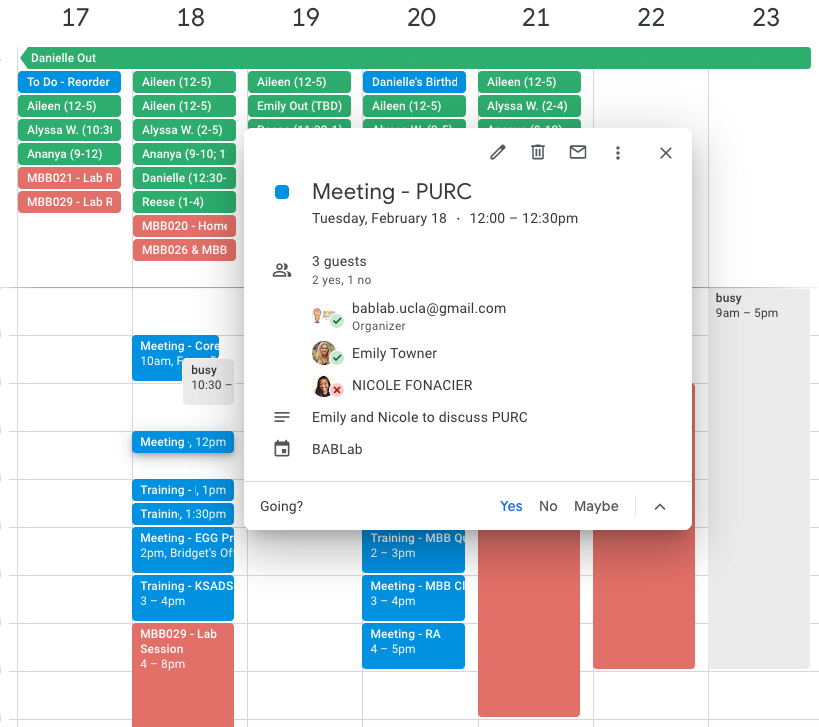
\includegraphics{images/lab_protocols/trainee_tuesdays_thursdays/1.png}
\caption{}
\end{figure}

I (Emily) have also shared my personal calendar with the BABLab account, so you can see when I am available to meet with you. You can access it by selecting ``Emily Towner'' from ``Other calendars'' in the BABLab calendar. The off-white ``busy'' slots are times I am unavailable (doctor's appointments, non lab-related meetings etc.).

\begin{figure}
\centering
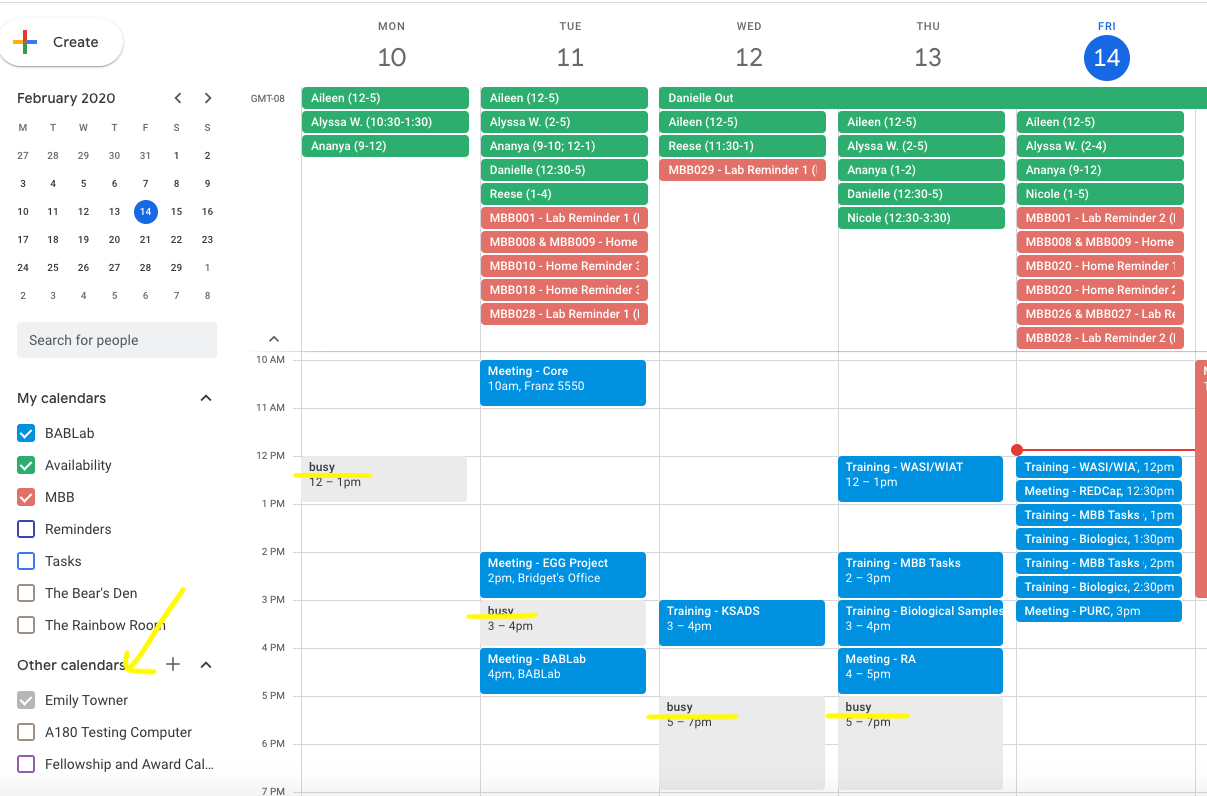
\includegraphics{images/lab_protocols/trainee_tuesdays_thursdays/2.png}
\caption{}
\end{figure}

\begin{center}\rule{0.5\linewidth}{\linethickness}\end{center}

\hypertarget{clinical-meetings}{%
\subsection{Clinical Meetings}\label{clinical-meetings}}

Purpose

The purpose of clinical meetings are to discuss and review ongoing clinical interviews (KSADs), troubleshoot any recent difficulties, and learn helpful interviewing tactics for future clinical interviews. During the meeting, you will present the team with background information from your clinical interview and walk through each supplement.

What To Prepare

Using a shared Dropbox Paper document, please prepare the following:

\begin{itemize}
\tightlist
\item
  Who you are presenting

  \begin{itemize}
  \tightlist
  \item
    Participant's KSADS file
  \item
    Date/time of session
  \end{itemize}
\item
  Brief background

  \begin{itemize}
  \tightlist
  \item
    Was the child bio/adopted?

    \begin{itemize}
    \tightlist
    \item
      Age of adoption
    \end{itemize}
  \item
    Was there any prenatal exposure?
  \item
    Any trouble in school?
  \end{itemize}
\item
  Supplements

  \begin{itemize}
  \tightlist
  \item
    Your thought process on why/why not you went through each supplements/diagnoses you have assigned
  \end{itemize}
\item
  Personal opinions

  \begin{itemize}
  \tightlist
  \item
    What was the child participant like in the session? (note relevant behaviors for context)
  \end{itemize}
\item
  WASI/WIAT

  \begin{itemize}
  \tightlist
  \item
    A quick overview of the participant's WASI/WIAT (admission and scores)
  \end{itemize}
\item
  Questions for the team

  \begin{itemize}
  \tightlist
  \item
    Any situations you feel may have been difficult to address during the clinical interview
  \end{itemize}
\end{itemize}

\emph{These meetings are also a safe space to debrief potentially difficult interviews.}

\begin{center}\rule{0.5\linewidth}{\linethickness}\end{center}

\hypertarget{mail}{%
\section{Mail}\label{mail}}

\begin{center}\rule{0.5\linewidth}{\linethickness}\end{center}

\hypertarget{usps}{%
\subsection{USPS}\label{usps}}

When sending things out USPS, you can place your recharge ID under the sender's address, circle it, \& drop it in the outgoing mail bin in 1282 (faculty mailroom)

\begin{center}\rule{0.5\linewidth}{\linethickness}\end{center}

\hypertarget{recycling-waste}{%
\section{Recycling \& Waste}\label{recycling-waste}}

We can leave small items outside our door for recycling/trash pickup. For large items we should bring them to the A-level loading dock to be recycled.

\begin{center}\rule{0.5\linewidth}{\linethickness}\end{center}

\hypertarget{purchasing}{%
\section{Purchasing}\label{purchasing}}

\begin{center}\rule{0.5\linewidth}{\linethickness}\end{center}

\hypertarget{pac-orders}{%
\subsection{PAC Orders}\label{pac-orders}}

PAC forms are used for most purchasing requests (besides Amazon which we can order from directly with our Amazon business account). Please consult the \href{http://staff.purchasing.ucla.edu/Portal/app/agreements/agreementsummary.aspx}{UCLA preferred vendors list} first before submitting a PAC form for an outside vendor.

\begin{itemize}
\tightlist
\item
  Save any quote to (BABLAB/Lab/Finances/Purchasing/)
\item
  Check Trello purchasing board for existing item
\item
  If no existing item, create one and add description based on templates
\item
  Fill out blank PAC form located in (BABLAB/Lab/Lab\_protocols/Finances/Purchasing/)
\item
  Save to (BABLAB/Lab/Finances/Purchasing)
\item
  Email the completed PAC order form to \href{mailto:psych-orders@psych.ucla.edu}{\nolinkurl{psych-orders@psych.ucla.edu}}

  \begin{itemize}
  \tightlist
  \item
    \textbf{Subject} - CB, {[}Fill in Vendor{]} Request, Bridget Callaghan
  \item
    CC' Bridget (\href{mailto:bcallaghan@ucla.edu}{\nolinkurl{bcallaghan@ucla.edu}}) - do not need signature if PI is cc'd
  \end{itemize}
\item
  Complete item order information on Trello purchasing board
\item
  Save PO (purchase order) and CONF (confirmation) if received
\item
  Once item is received lab manager log amount in funds spreadsheet

  \begin{itemize}
  \tightlist
  \item
    Add in any tax/shipping/expense that wasn't accounted for on Trello to most expensive item
  \item
    Mark as ``Logged'' on Trello
  \end{itemize}
\end{itemize}

\begin{center}\rule{0.5\linewidth}{\linethickness}\end{center}

\hypertarget{amazon-orders}{%
\subsection{Amazon Orders}\label{amazon-orders}}

Instructions for checking out via our Amazon Business Account.

\begin{itemize}
\tightlist
\item
  Check for existing item on Trello
\item
  If existing item, move to ``To Order'' list, change label to not logged, and create new instance of purchase in description box
\item
  To checkout via Amazon, Choose a Group

  \begin{itemize}
  \tightlist
  \item
    Upon clicking ``Proceed to Checkout'' you will arrive to the screen below. Select your fund manager's group and click continue:
  \item
    Be sure to select the correct group to avoid your order being rejected or sitting in a queue that is not being reviewed. In the event that your fund manager is out of the office, please check with the Business Office before starting your Amazon Business order so that we can add you to another group temporarily. Otherwise, the order will remain in your fund manager's queue until they are back in the office and able to approve orders.
  \end{itemize}
\item
  Business Order Information

  \begin{itemize}
  \tightlist
  \item
    Enter the Full Accounting Unit (FAU) or Recharge ID in the Purchase Order (PO) Number field and enter a business justification in the Comments for Approver field. These fields are required for the Psychology Department. If this information is not provided, your fund manager will reject the order.
  \item
    NOTE: Business justifications must describe the purpose of items being purchased, how and where the items will be used. Please be sure to be as detailed and specific as possible. If you are purchasing an item flagged as restricted your fund manager may reach out to you for additional information.\\
  \item
    Restricted items are not necessarily unallowable, but may require additional levels of approval from the Pcard Administrator in Purchasing before we can charge it to a Pcard.
  \end{itemize}
\item
  Next, select the appropriate shipping address
\item
  Next, you will select the method of payment. This should be a VISA with your fund manager's name on the card. You do not have the option to edit this page and it is not necessary to include a reference number. Click continue.
\item
  Review your order details and once confirmed, click on submit order for approval.
\item
  Complete item order information on Trello and move to ``Submitted'' list
\item
  Once placed, move item to ``Placed'' list on Trello
\item
  Once item is received, lab manager to log amount in funds spreadsheet

  \begin{itemize}
  \tightlist
  \item
    Add in any tax/shipping/expense that wasn't accounted for on Trello to most expensive item
  \item
    Mark as ``Logged'' on Trello
  \end{itemize}
\end{itemize}

\begin{center}\rule{0.5\linewidth}{\linethickness}\end{center}

\hypertarget{reimbursement}{%
\subsection{Reimbursement}\label{reimbursement}}

For reimbursement:

\begin{itemize}
\tightlist
\item
  Fill out a blank reimbursement form found in (BABLAB/Lab/Lab\_protocols/Finances/Reimbursement/)
\item
  Save reimbursement form to (BABLAB/Lab/Finances/Reimbursement)
\item
  Email the completed reimbursement form to \href{mailto:psych-orders@psych.ucla.edu}{\nolinkurl{psych-orders@psych.ucla.edu}}

  \begin{itemize}
  \tightlist
  \item
    Subject - CB, {[}Fill in Vendor{]} Reimbursement, Bridget Callaghan
  \item
    CC' Bridget (\href{mailto:bcallaghan@ucla.edu}{\nolinkurl{bcallaghan@ucla.edu}}) - do not need signature if PI is cc'd
  \end{itemize}
\item
  Lab manager log reimbursement amount in funds spreadsheet
\end{itemize}

\begin{center}\rule{0.5\linewidth}{\linethickness}\end{center}

\hypertarget{guest-parking-passes}{%
\subsection{Guest Parking Passes}\label{guest-parking-passes}}

\begin{itemize}
\tightlist
\item
  Email Tyler Tuione (\href{mailto:tuione@psych.ucla.edu}{\nolinkurl{tuione@psych.ucla.edu}}) saying you would like to purchase guest parking passes.
\item
  Information to include in this email:

  \begin{itemize}
  \tightlist
  \item
    Number of passes to order
  \item
    Recharge ID for fund to charge
  \end{itemize}
\item
  Wait for Parking Services to call the lab (about a week), record the confirmation code they give you.
\item
  Pick up the passes with the confirmation code at 555 Westwood Plaza, Suite 100.
\end{itemize}

\begin{center}\rule{0.5\linewidth}{\linethickness}\end{center}

\hypertarget{petty-cash}{%
\subsection{Petty Cash}\label{petty-cash}}

\begin{itemize}
\tightlist
\item
  Fill out a blank IRB research payment request form (for cash or card)(BABLAB/Lab/Lab\_protocols/Finances/Petty\_cash/)
\item
  Send it to Brian Hoang (\href{mailto:brianhoang@psych.ucla.edu}{\nolinkurl{brianhoang@psych.ucla.edu}}) for a signature
\item
  Submit the form at this \href{https://sa.ucla.edu/MessageCenter/OneStop/Home/PostMessage?topicId=293}{site}
\item
  It can take up to 10 business days for them to reply back.
\item
  When they recontact with a delivery time, ensure that either of the people who signed the form (Bridget and an RA) are in the lab at the time of delivery to sign off on the order.
\item
  They will not deliver the cash if one of the signers is not present
\item
  Once the disbursement is received, log it on the study specific payment log
\item
  Ask the lab manager to log the pettycash amount in the funds spreadsheet
\end{itemize}

\begin{center}\rule{0.5\linewidth}{\linethickness}\end{center}

\hypertarget{vendor-specific-protocols}{%
\subsection{Vendor specific protocols}\label{vendor-specific-protocols}}

Some vendors have special requirements or instructions to make purchases from them.

Biopac
- Email \href{mailto:aimeew@biopac.com}{\nolinkurl{aimeew@biopac.com}} and \href{mailto:frontdesk@biopac.com}{\nolinkurl{frontdesk@biopac.com}}

Uprinting

\begin{itemize}
\tightlist
\item
  Go to Uprinting.com and log in.
\item
  Select the items you want to purchase and add them to the cart.

  \begin{itemize}
  \tightlist
  \item
    Note that you need to have the pdf or image files on-hand and make sure they match the dimensions of what they will be printed on
  \end{itemize}
\item
  When checking out, select ``Terms'' as the payment method
\item
  Create and submit a PAC form to purchasing as usual, but also cc' \href{mailto:jhoan.e@digitalroominc.com}{\nolinkurl{jhoan.e@digitalroominc.com}} and request that purchasing get in touch with her to pay for the order
\end{itemize}

\begin{center}\rule{0.5\linewidth}{\linethickness}\end{center}

\hypertarget{logging-purchases-on-trello}{%
\subsection{Logging purchases on Trello}\label{logging-purchases-on-trello}}

\begin{enumerate}
\def\labelenumi{\arabic{enumi}.}
\tightlist
\item
  Go to the ``Purchasing'' board on Trello. It should be green.There are different tabs:
\end{enumerate}

\begin{itemize}
\tightlist
\item
  \textbf{To Return}: items that will be returned
\item
  \textbf{Maybe}: items that may be bought
\item
  \textbf{To Order}: items to order/ buy
\item
  \textbf{Submitted}: orders that have been submitted
\item
  \textbf{Placed}: orders that have been placed
\item
  \textbf{In Stock}: items that have arrived and are in lab
\end{itemize}

\begin{enumerate}
\def\labelenumi{\arabic{enumi}.}
\setcounter{enumi}{1}
\item
  Add a card to ``To Order'' - name it with this format: \textbf{item being bought - \$price}
\item
  Add the following labels:
\end{enumerate}

\begin{itemize}
\tightlist
\item
  \textbf{Budget: Nonlogged} (always log this by default)
\item
  \textbf{Fund} (ask lab manager whether it's Startup, R00, or other fund)
\item
  \textbf{Category} (ask lab manager which category)
\end{itemize}

\begin{enumerate}
\def\labelenumi{\arabic{enumi}.}
\setcounter{enumi}{3}
\item
  Add the link of the item on `add an attachment'. Rename the link the exact name of the item as written on Amazon (or whatever website).
\item
  Add a description with this format:
\end{enumerate}

\begin{itemize}
\tightlist
\item
  Units: (insert amount of item, ex. 20 pencils)
\item
  Orders: (insert how many orders placed, ex. 1 order of 20 pencils)
\item
  Date submitted: (insert date we submitted order)
\item
  Date placed: (insert date vendor has placed order)
\item
  Date received: (insert date we got it in lab)
\item
  If the card is something that may run out eventually (ex. granola bars, notebooks) add an approximate due date.
\end{itemize}

\begin{enumerate}
\def\labelenumi{\arabic{enumi}.}
\setcounter{enumi}{5}
\tightlist
\item
  Whenever an item has been submitted, placed, and in stock, move the card into its respective tab.
\end{enumerate}

Watch the video for a detailed explanation.

\begin{center}\rule{0.5\linewidth}{\linethickness}\end{center}

\hypertarget{technology}{%
\section{Technology}\label{technology}}

\begin{center}\rule{0.5\linewidth}{\linethickness}\end{center}

\hypertarget{slack}{%
\subsection{Slack}\label{slack}}

If you haven't already found this out for yourself, emails are a clunky way of communicating for most lab needs. Moreover, most people will find that they have a backlog of emails awaiting their attention. For this reason, we will use Slack for the primary means of lab communication.

The beauty of Slack is that you only subscribe to the channels that concern you. For messages to one person or a small group, use direct messages. If you have to include out-of-lab recipients, use e-mail. If you have a paper you want to share, download it and then upload it to Slack in the \#papers channel.

Full-time lab members should install Slack on their computers and/or phones and check it regularly (during working hours). Part-time lab members should also check Slack when they are working in the lab as there may be important messages in there for them.

Of course, if there is an emergency, and you need to contact Bridget, use her email or phone or drop into her office.

\begin{longtable}[]{@{}lll@{}}
\toprule
\begin{minipage}[b]{0.18\columnwidth}\raggedright
Slack Channel\strut
\end{minipage} & \begin{minipage}[b]{0.04\columnwidth}\raggedright
Type\strut
\end{minipage} & \begin{minipage}[b]{0.70\columnwidth}\raggedright
Purpose\strut
\end{minipage}\tabularnewline
\midrule
\endhead
\begin{minipage}[t]{0.18\columnwidth}\raggedright
\#bablab\_core\strut
\end{minipage} & \begin{minipage}[t]{0.04\columnwidth}\raggedright
Private\strut
\end{minipage} & \begin{minipage}[t]{0.70\columnwidth}\raggedright
For private communication between the core team - this includes the PI, Lab Managers, Postdocs, and Grad Students\strut
\end{minipage}\tabularnewline
\begin{minipage}[t]{0.18\columnwidth}\raggedright
\#bablab\_ra\strut
\end{minipage} & \begin{minipage}[t]{0.04\columnwidth}\raggedright
Private\strut
\end{minipage} & \begin{minipage}[t]{0.70\columnwidth}\raggedright
For private communication between the lab managers and all the research assistants\strut
\end{minipage}\tabularnewline
\begin{minipage}[t]{0.18\columnwidth}\raggedright
\#bablab\_senior\_ra\strut
\end{minipage} & \begin{minipage}[t]{0.04\columnwidth}\raggedright
Private\strut
\end{minipage} & \begin{minipage}[t]{0.70\columnwidth}\raggedright
For private communication between the lab managers and the senior research assistants\strut
\end{minipage}\tabularnewline
\begin{minipage}[t]{0.18\columnwidth}\raggedright
\#general\strut
\end{minipage} & \begin{minipage}[t]{0.04\columnwidth}\raggedright
Public\strut
\end{minipage} & \begin{minipage}[t]{0.70\columnwidth}\raggedright
For lab-wide communication and announcements\strut
\end{minipage}\tabularnewline
\begin{minipage}[t]{0.18\columnwidth}\raggedright
\#meetings\_lab\strut
\end{minipage} & \begin{minipage}[t]{0.04\columnwidth}\raggedright
Public\strut
\end{minipage} & \begin{minipage}[t]{0.70\columnwidth}\raggedright
For notes or communication related to lab meetings\strut
\end{minipage}\tabularnewline
\begin{minipage}[t]{0.18\columnwidth}\raggedright
\#methods\_fmri\strut
\end{minipage} & \begin{minipage}[t]{0.04\columnwidth}\raggedright
Public\strut
\end{minipage} & \begin{minipage}[t]{0.70\columnwidth}\raggedright
Sharing wisdom on fMRI data collection / analysis or asking (and answering) the fMRI questions of others\strut
\end{minipage}\tabularnewline
\begin{minipage}[t]{0.18\columnwidth}\raggedright
\#methods\_mb\strut
\end{minipage} & \begin{minipage}[t]{0.04\columnwidth}\raggedright
Public\strut
\end{minipage} & \begin{minipage}[t]{0.70\columnwidth}\raggedright
Sharing wisdom on microbiome data collection / analysis or asking and answering the microbiome questions of others\strut
\end{minipage}\tabularnewline
\begin{minipage}[t]{0.18\columnwidth}\raggedright
\#notes\_conferences\strut
\end{minipage} & \begin{minipage}[t]{0.04\columnwidth}\raggedright
Public\strut
\end{minipage} & \begin{minipage}[t]{0.70\columnwidth}\raggedright
For taking notes at conferences\strut
\end{minipage}\tabularnewline
\begin{minipage}[t]{0.18\columnwidth}\raggedright
\#papers\strut
\end{minipage} & \begin{minipage}[t]{0.04\columnwidth}\raggedright
Public\strut
\end{minipage} & \begin{minipage}[t]{0.70\columnwidth}\raggedright
Sharing links to lab-relevant papers and discussing them\strut
\end{minipage}\tabularnewline
\begin{minipage}[t]{0.18\columnwidth}\raggedright
\#random\strut
\end{minipage} & \begin{minipage}[t]{0.04\columnwidth}\raggedright
Public\strut
\end{minipage} & \begin{minipage}[t]{0.70\columnwidth}\raggedright
Non-work-related chatting -- e.g., pics of pets, funny cartoons etc.\strut
\end{minipage}\tabularnewline
\begin{minipage}[t]{0.18\columnwidth}\raggedright
\#recruitment\strut
\end{minipage} & \begin{minipage}[t]{0.04\columnwidth}\raggedright
Public\strut
\end{minipage} & \begin{minipage}[t]{0.70\columnwidth}\raggedright
Any ideas you have for recruiting youth into our study\strut
\end{minipage}\tabularnewline
\begin{minipage}[t]{0.18\columnwidth}\raggedright
\#stats\strut
\end{minipage} & \begin{minipage}[t]{0.04\columnwidth}\raggedright
Public\strut
\end{minipage} & \begin{minipage}[t]{0.70\columnwidth}\raggedright
To ask and answer questions about statistical analyses\strut
\end{minipage}\tabularnewline
\begin{minipage}[t]{0.18\columnwidth}\raggedright
\#study\_egg\_emotionality\strut
\end{minipage} & \begin{minipage}[t]{0.04\columnwidth}\raggedright
Private\strut
\end{minipage} & \begin{minipage}[t]{0.70\columnwidth}\raggedright
To discuss issues related to the EGG and Emotionality study\strut
\end{minipage}\tabularnewline
\begin{minipage}[t]{0.18\columnwidth}\raggedright
\#study\_mbb\strut
\end{minipage} & \begin{minipage}[t]{0.04\columnwidth}\raggedright
Private\strut
\end{minipage} & \begin{minipage}[t]{0.70\columnwidth}\raggedright
To discuss issues related to the Mind, Brain, Body study\strut
\end{minipage}\tabularnewline
\begin{minipage}[t]{0.18\columnwidth}\raggedright
\#study\_transfer\_mental\_health\strut
\end{minipage} & \begin{minipage}[t]{0.04\columnwidth}\raggedright
Private\strut
\end{minipage} & \begin{minipage}[t]{0.70\columnwidth}\raggedright
To discuss issues related to the Transfer Mental Health Study\strut
\end{minipage}\tabularnewline
\begin{minipage}[t]{0.18\columnwidth}\raggedright
\#tips\_coding\strut
\end{minipage} & \begin{minipage}[t]{0.04\columnwidth}\raggedright
Public\strut
\end{minipage} & \begin{minipage}[t]{0.70\columnwidth}\raggedright
Sharing wisdom on code writing or asking (and answering) the coding questions of others\strut
\end{minipage}\tabularnewline
\bottomrule
\end{longtable}

\begin{center}\rule{0.5\linewidth}{\linethickness}\end{center}

\hypertarget{box}{%
\subsection{Box}\label{box}}

We have moved over to Box for our file storage service. This works very similarly to Google Drive or Dropbox, but is more secure. Additionally, each lab member can have their own account, it's free and great for collaboration!

Please download \href{https://www.box.com/drive}{Box Drive} to use.

\begin{enumerate}
\def\labelenumi{\arabic{enumi}.}
\tightlist
\item
  Click download for your operating system
\end{enumerate}

\begin{figure}
\centering
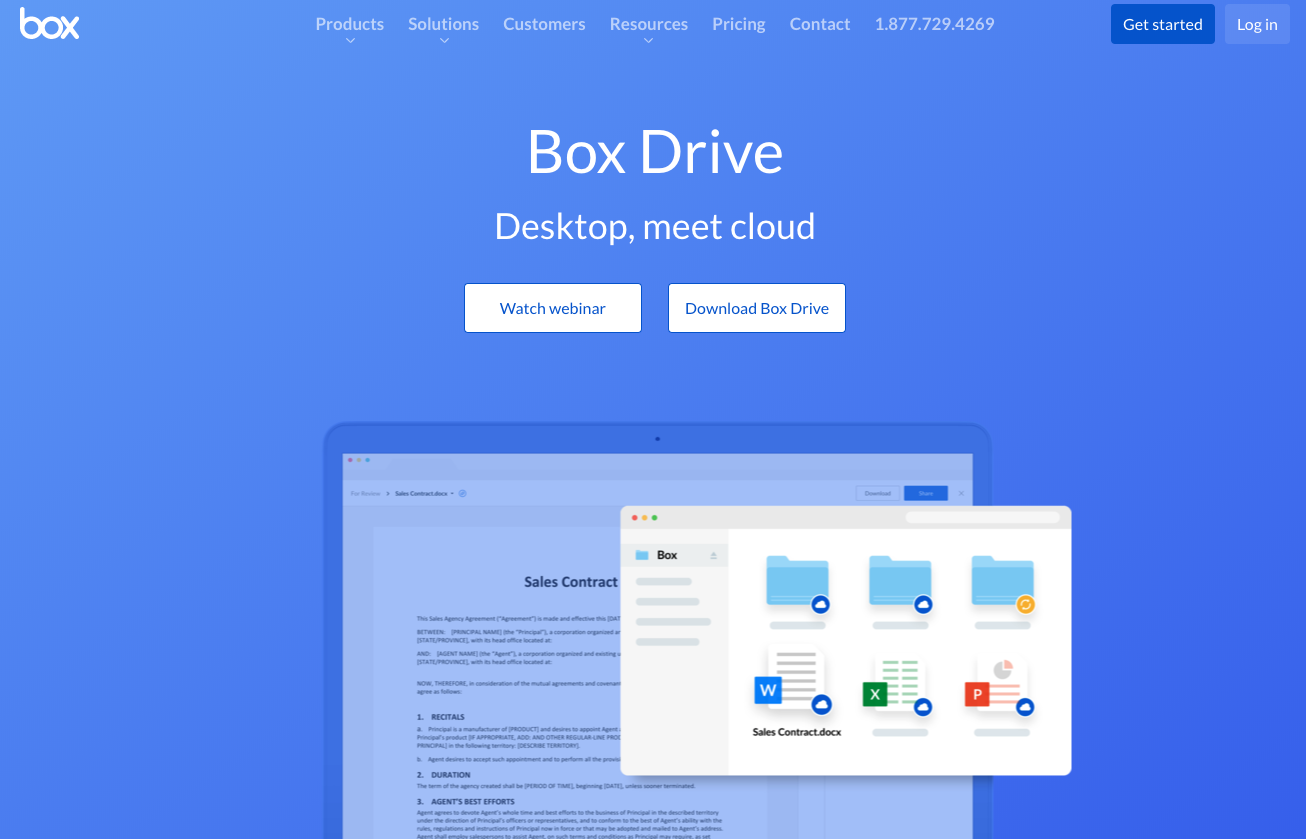
\includegraphics{images/lab_protocols/box/1.png}
\caption{}
\end{figure}

\begin{enumerate}
\def\labelenumi{\arabic{enumi}.}
\setcounter{enumi}{1}
\tightlist
\item
  After installing, you may need to click allow in your security preferences
\end{enumerate}

\begin{figure}
\centering
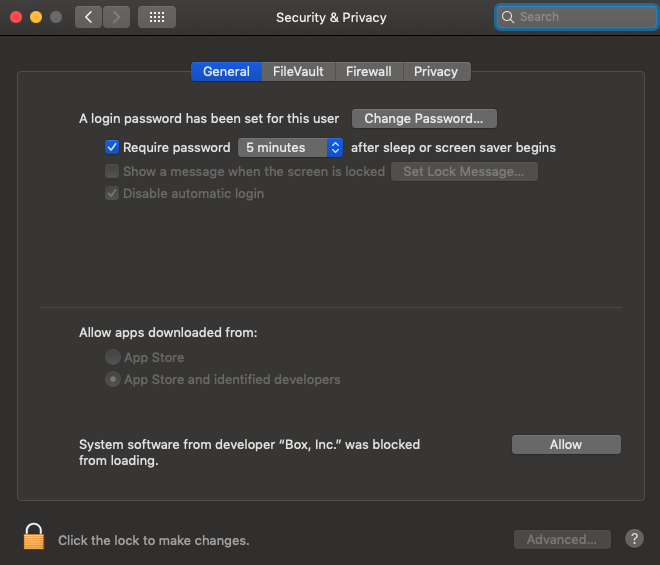
\includegraphics{images/lab_protocols/box/2.png}
\caption{}
\end{figure}

\begin{enumerate}
\def\labelenumi{\arabic{enumi}.}
\setcounter{enumi}{2}
\tightlist
\item
  Log in with your UCLA email (make sure to accept the Box sharing request first)
\end{enumerate}

\begin{figure}
\centering
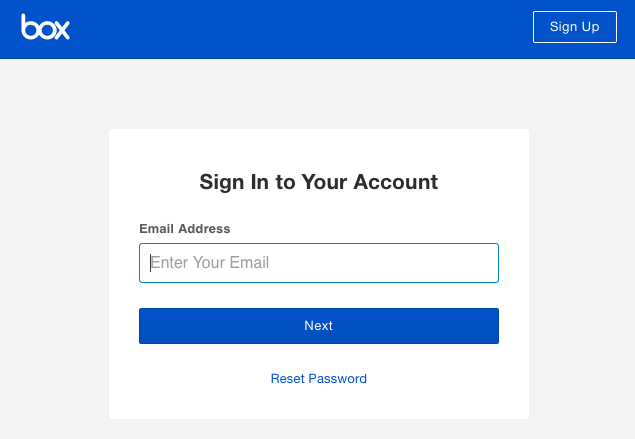
\includegraphics{images/lab_protocols/box/3.png}
\caption{}
\end{figure}

\begin{enumerate}
\def\labelenumi{\arabic{enumi}.}
\setcounter{enumi}{3}
\tightlist
\item
  Now you can use Box on your desktop.
\end{enumerate}

\begin{figure}
\centering
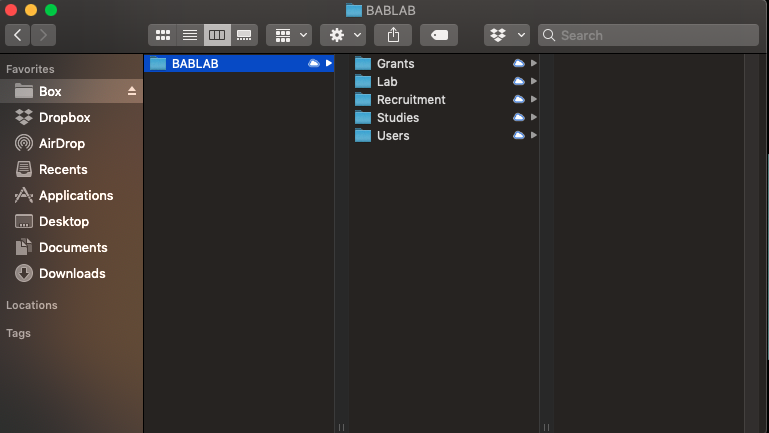
\includegraphics{images/lab_protocols/box/4.png}
\caption{}
\end{figure}

\begin{enumerate}
\def\labelenumi{\arabic{enumi}.}
\setcounter{enumi}{4}
\tightlist
\item
  On the web version, change your notification preferences so that you don't get an email every time someone uploads a file by unchecking the boxes below
\end{enumerate}

\begin{figure}
\centering
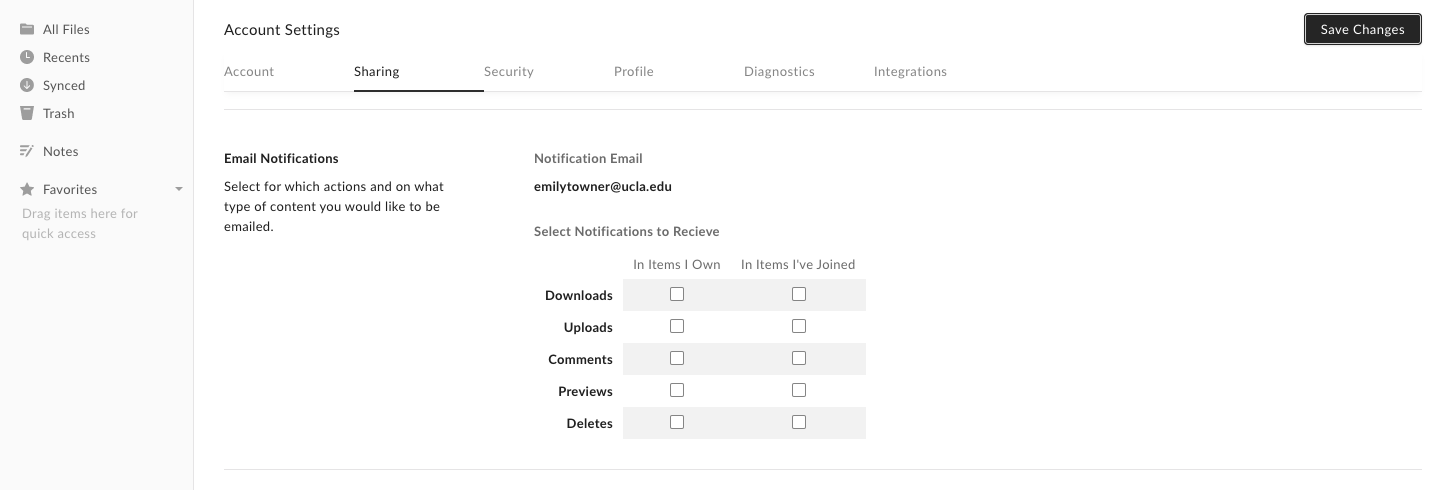
\includegraphics{images/lab_protocols/box/5.png}
\caption{}
\end{figure}

\begin{center}\rule{0.5\linewidth}{\linethickness}\end{center}

\hypertarget{using-trello}{%
\subsection{Using Trello}\label{using-trello}}

\begin{enumerate}
\def\labelenumi{\arabic{enumi}.}
\tightlist
\item
  There are multiple lists on the Tasks Board!
  These include: Doing, To-do, Later and Done.
  Depending on the task, simply move it to the right list once you progress with it.
\end{enumerate}

\begin{itemize}
\tightlist
\item
  \textbf{To Do:} Current tasks to complete.
\item
  \textbf{Doing:} Tasks currently being done.
\item
  \textbf{Later}: Tasks not as pressing, but still must be done.
\item
  \textbf{Done}: Completed tasks.
\end{itemize}

\begin{enumerate}
\def\labelenumi{\arabic{enumi}.}
\setcounter{enumi}{1}
\tightlist
\item
  \textbf{To add a card}: Click `+ Add Another Card' under the appropriate list. There are multiple functions within this:
\end{enumerate}

\begin{itemize}
\tightlist
\item
  You can add members, labels (useful for studies), checklist, attachment, due date and more to the back of the card. This information will show when you click on the card.
\end{itemize}

\begin{enumerate}
\def\labelenumi{\arabic{enumi}.}
\setcounter{enumi}{2}
\tightlist
\item
  \textbf{Show Menu function:} This is a great way to search specific items, such as your own name for tasks, or the study for which there are tasks for, or tasks which have upcoming due dates.
\end{enumerate}

\begin{center}\rule{0.5\linewidth}{\linethickness}\end{center}

\hypertarget{server}{%
\subsection{Server}\label{server}}

In addition to Box, we make regular biweekly backups to a dedicated psychology department server (in addition to two external drives)

To connect to the CallaghanLab server:

*Contact the lab manager first to set up your credentials.

On a Mac --

\begin{itemize}
\tightlist
\item
  From the dropdown menu under ``Go'', select ``Connect to Server\ldots{}'' (Apple + K)
\item
  Enter the network/server address: \texttt{smb://pythia.psych.ucla.edu/Users/CallaghanLab/}
\item
  Click on ``Connect''.
\item
  A dialogue box will prompt you for your credentials. Enter your credentials obtained from Psychology IT and click on ``OK''.
\item
  If everything was entered correctly from above, the mapped drive will appear under ``Shared'' in the Mac's Finder.
\end{itemize}

On a PC --

\begin{itemize}
\tightlist
\item
  From the Windows file explorer, right mouse click on ``Computer'' for Windows 7 or ``This PC'' on Windows 8/10.
\item
  Select ``Map network drive''.
\item
  Specify an available ``Drive'' letter from the dropdown menu.
\item
  Enter the network/server location for the ``Folder'' field and click on ``Finish''.

  \begin{itemize}
  \tightlist
  \item
    Network/server location: \texttt{\textbackslash{}\textbackslash{}pythia.psych.ucla.edu\textbackslash{}Users\textbackslash{}CallaghanLab\textbackslash{}}
  \end{itemize}
\item
  Enter your username and password that was provided by Psychology IT in the ``network credentials'' popup dialogue box and click on OK.
\item
  If everything was entered correctly from above, the mapped drive will appear under ``Network locations'' when you click on ``Computer/This PC''.
\item
  After the drive has been mapped, logged out of Windows to ``logout'' from the network drive.
\item
  Don't right mouse click on the mapped drive and select ``Disconnect''. This will only unmap the network drive and you will have to go through the process all over again.
\end{itemize}

To connect off-campus connect to the UCLA/BOL VPN and let it run in the background prior to logging into the mapped drive you had configured on your computer.

How-to download/install the \href{https://help.bol.ucla.edu/kb_view.do?sysparm_article=kb0010923}{Cisco VPN client}.

\begin{quote}
Every night the server is backed up to the Life Sciences data center in Hershey Hall. That's always been the case. To make those nightly backups more safe, there is another copy of the backups stored offsite (i.e.~to prevent losing both the server AND the backups in a fire, earthquake, etc.)

Once we have Shadow Copy enabled, we'll also have more direct access to backups, so we won't need to work with Life Sciences to retrieve backups. Psych IT will be able to grab a recent copy of your files/folders ourselves. We'll also have access to incremental backups (i.e.~yesterday's copy, two day old copy, three day old copy\ldots{}up to two weeks back).

So at that point we'll have 3 forms of backup, and plenty of safety net.

\begin{itemize}
\tightlist
\item
  Dave (Psych IT)
\end{itemize}
\end{quote}

\begin{center}\rule{0.5\linewidth}{\linethickness}\end{center}

\hypertarget{dropbox-paper}{%
\subsection{Dropbox Paper}\label{dropbox-paper}}

The lab has a shared Dropbox Paper account --- which is slightly different than regular Dropbox file storage. On the Dropbox Paper, we will place collaborative documents. We will grant you access permission to various folders in the Dropbox Paper account, You may need to initialize an account with the email we grant access permission.

\begin{center}\rule{0.5\linewidth}{\linethickness}\end{center}

\hypertarget{github}{%
\subsection{GitHub}\label{github}}

The lab's GitHub should be used to share code and data with people outside of the lab (i.e., people not on our IRB). Not all data can be shared (because of IRB restrictions) and not all data that can be shared should be shared immediately. Speak with Bridget about when to share data, and what needs to be done to the data (e.g., the level of de-identification required) before we share it. Ask the lab manager to get access to the lab's GitHub.

Our lab manual, lab wiki, and study wikis are also hosted on our GitHub.

\begin{center}\rule{0.5\linewidth}{\linethickness}\end{center}

\hypertarget{google-calendars}{%
\subsection{Google Calendars}\label{google-calendars}}

The lab has many Google calendars and you should subscribe to those that make sense for your unique situation.

\begin{enumerate}
\def\labelenumi{\arabic{enumi}.}
\tightlist
\item
  \textbf{BABLab:} Used for lab meetings, out of schedule meetings, birthdays, formal lab events etc.
\item
  \textbf{Availability:} If you are part time, please place the hours you plan to come into the lab on this calendar. If you are going to be away, please place the dates and times on this calendar. This is critical as the lab manager will use this information when scheduling people to run participants for our studies. Bridget and the core team will also put her out of office times on this calendar to help people with scheduling.\\
\item
  \textbf{MBB:} Used for booking sessions and reminders for the Mind, Brain, Body study
\item
  \textbf{The Bear's Den:} used to reserve time in experimental room 1
\item
  \textbf{The Rainbow Room:} used to reserve time in experimental room 2
\item
  \textbf{A180 Testing Computer:} the SAND Lab room that can be used for blood spots
\item
  \textbf{HPL1333:} The Health Psychology Lab room that can be used for blood spots
\end{enumerate}

\begin{center}\rule{0.5\linewidth}{\linethickness}\end{center}

\hypertarget{e-mail}{%
\subsection{E-mail}\label{e-mail}}

We have an email listserv for communicating with the whole lab and individuals who subscribe to our list - including visitors and students from other labs who attend our meetings, visiting scholars, etc.

The email is: \textbf{\href{mailto:bablab@googlegroups.com}{\nolinkurl{bablab@googlegroups.com}}}

If you are thinking about joining the lab and would like to be notified about upcoming lab meetings, please request to join the listserv.

There is also a lab email account which people use to contact the lab to participate in studies (\href{mailto:bablab.ucla@gmail.com}{\nolinkurl{bablab.ucla@gmail.com}}). This email account will be staffed by the lab manager/s and they will sort the emails in specific folders within the Gmail account. If you are running a study, it is your responsibility to check your study's folder on the lab Gmail every few days and respond to participant inquiries in the ``potential'' participants folder in relation to your study.

\begin{center}\rule{0.5\linewidth}{\linethickness}\end{center}

\hypertarget{mac-os---catalina}{%
\subsection{Mac OS - Catalina}\label{mac-os---catalina}}

If you upgrade your Mac operating system to Catalina, and wish to run tasks on PsychoPy, you must enable the following settings in the image below.

\begin{figure}
\centering
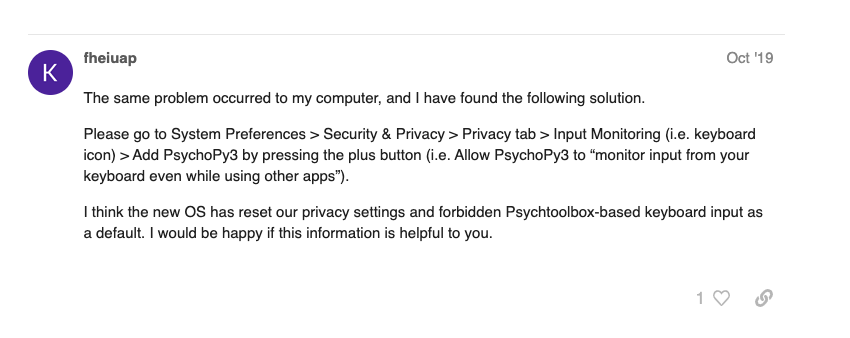
\includegraphics{images/lab_protocols/catalina/1.png}
\caption{}
\end{figure}

\begin{center}\rule{0.5\linewidth}{\linethickness}\end{center}

\hypertarget{redcap}{%
\subsection{REDCap}\label{redcap}}

\hypertarget{entering-instruments}{%
\subsubsection{Entering Instruments}\label{entering-instruments}}

\begin{center}\rule{0.5\linewidth}{\linethickness}\end{center}

\hypertarget{equipment}{%
\section{Equipment}\label{equipment}}

\begin{center}\rule{0.5\linewidth}{\linethickness}\end{center}

\hypertarget{biopac}{%
\subsection{Biopac}\label{biopac}}

\begin{center}\rule{0.5\linewidth}{\linethickness}\end{center}

\hypertarget{printer}{%
\subsection{Printer}\label{printer}}

\begin{itemize}
\tightlist
\item
  Make sure you are connected to eduroam wifi
\item
  Open up Printer \& Scanners in System Preferences

  \begin{itemize}
  \tightlist
  \item
    If current printer is not working, right click printer and click Reset Printing System
    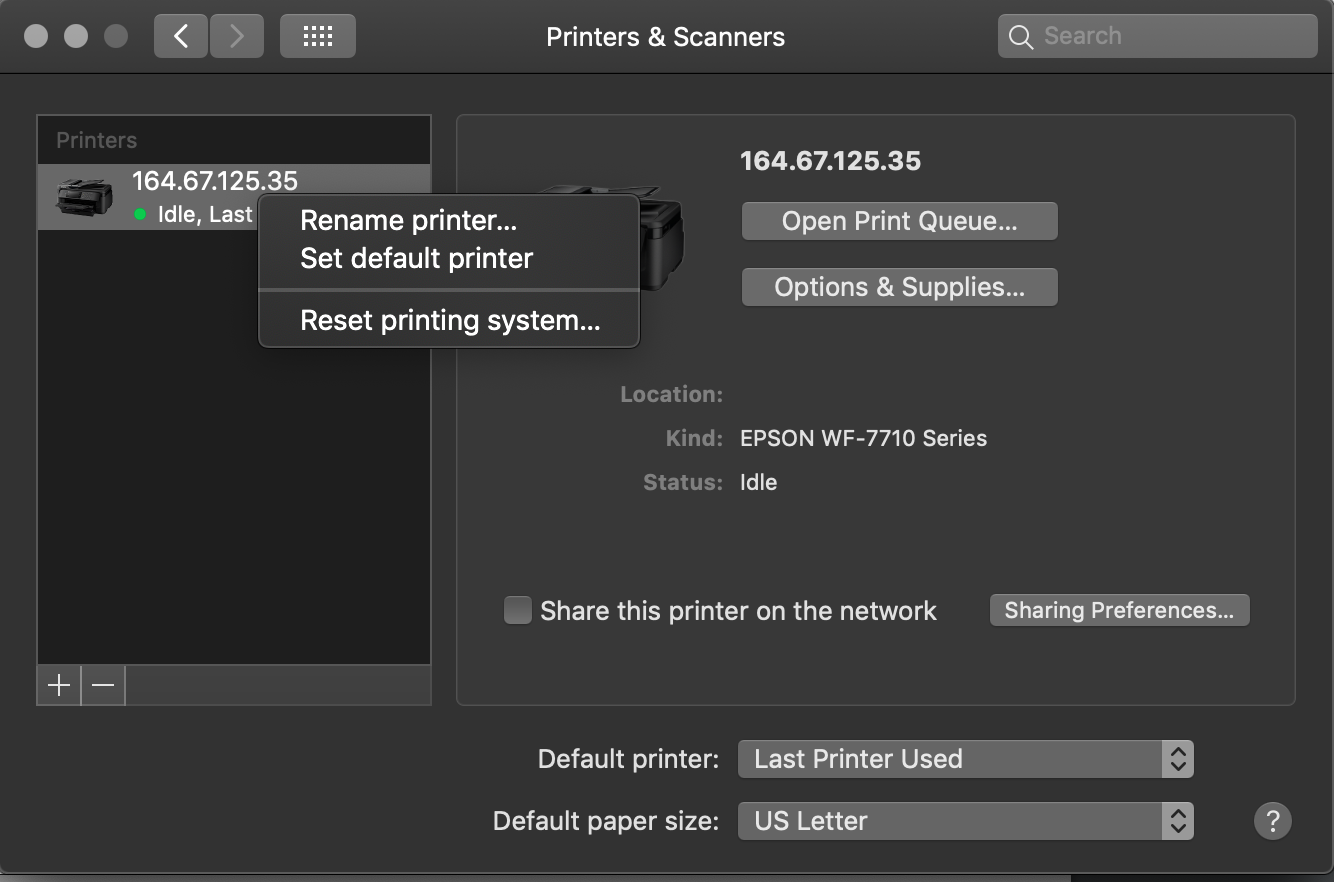
\includegraphics{images/lab_protocols/printer/1.png}
  \end{itemize}
\item
  Reset Computer
\item
  Open up System Preferences -- Printers \& Scanners
\item
  Click on + sign to add a printer
\item
  Enter IP Address from Printer: 164.67.125.35
  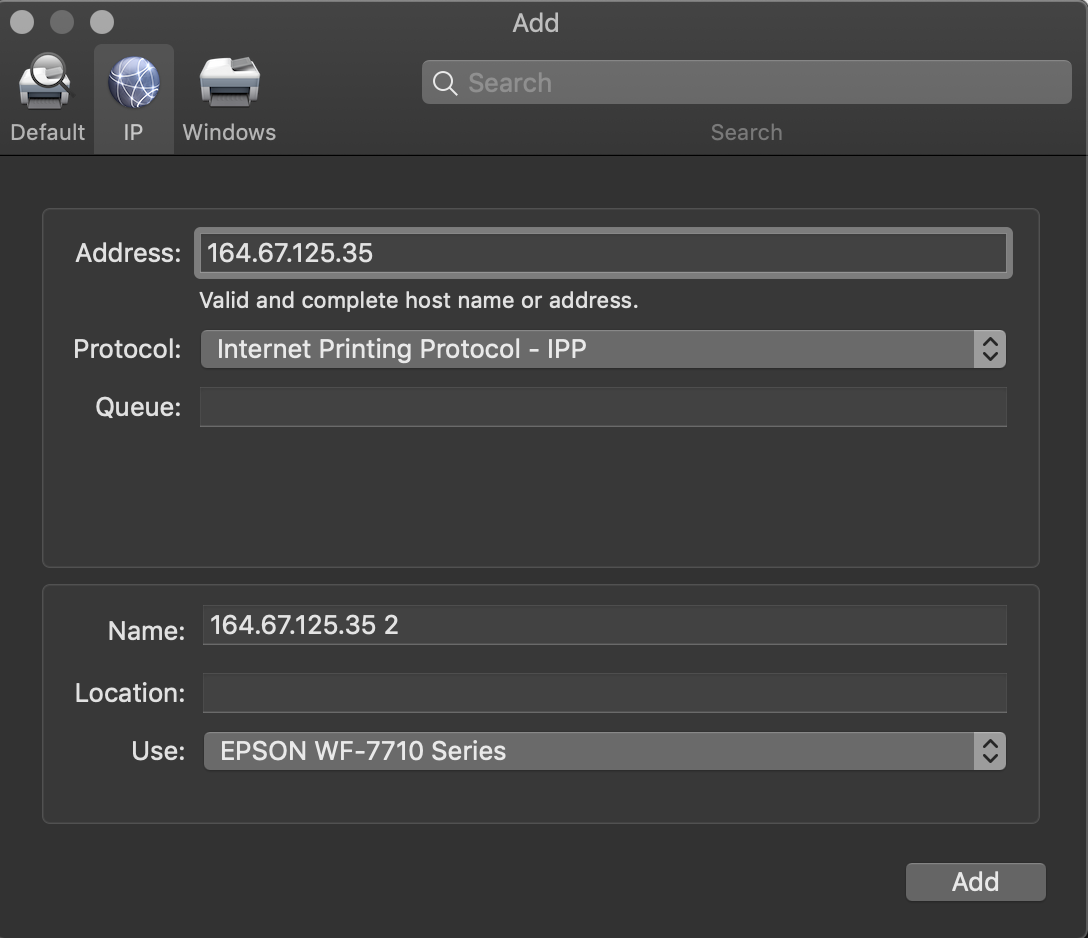
\includegraphics{images/lab_protocols/printer/2.png}
\item
  Make sure Use displays: EPSON WF-7710 Series
\item
  Click ADD
\item
  Reset your Printer Presets if needed
\end{itemize}

\begin{center}\rule{0.5\linewidth}{\linethickness}\end{center}

\hypertarget{social-media}{%
\section{Social Media}\label{social-media}}

\begin{center}\rule{0.5\linewidth}{\linethickness}\end{center}

\hypertarget{instagram}{%
\subsection{Instagram}\label{instagram}}

The pride and joy of the lab. There is a lot of content to keep track of and to ensure is posted weekly.

General important rules:

\begin{itemize}
\tightlist
\item
  Keep posts short, family-friendly, and accessible.
\item
  If you post on the story, it should also likely be added to a story highlight.
\item
  Stick to the color scheme and aesthetic (this includes matching the text in story highlights to the story highlight cover color).
\item
  Maintain the integrity of the main feed grid (will be elaborated on further down).
\item
  Maintain the consistency of the Lab's hashtags (will be elaborated on further down).
\end{itemize}

Feed Content:

\begin{itemize}
\tightlist
\item
  The feed grid is an important part of the aesthetic of the lab's social media. We can divide the grid into ``A Week'' and ``B Week'' rows. Because there are 3 posts horizontally in the grid, there should be 3 pieces of content posted each week (or with relative consistency).
\end{itemize}

``A Week'':

\begin{itemize}
\tightlist
\item
  Biome Bites! ad post: This is simply a post saying to check the story for this week's Biome Bites! installment. The caption for this should be brief and maybe reference the content in the actual story post.
\item
  Lab Meeting ad post OR Email List ad post: Post this on lab meeting day in ``A Week''. If there is a speaker or specific topic for the week, discuss that briefly in the caption.
\item
  In ``B Week'', don't post this even if there is a lab meeting. Instead, post a previous Lab Meeting ad post on the story. If there is not a lab meeting during that ``A Week'', you should post the Email List ad post instead.
\item
  Brain Bites! ad post: This is simply a post saying to check the story for this week's Brain Bites! installment. The caption for this should be brief and maybe reference the content in the actual story post.
\end{itemize}

``B Week'':

\begin{itemize}
\tightlist
\item
  3 random posts: post pictures from around the lab, from events, or advertisements for upcoming events. Check the existing feed for ideas, and try to stay current with seasons, trends, etc.
\item
  If there is an event upcoming, use the following template to advertise it.
\end{itemize}

Important notes for all feed content:

\begin{itemize}
\tightlist
\item
  Post all posts to both instagram and facebook (integrated feature on insta)
\item
  End every single post with the following: \#brain
\item
  Add 2-3 topical hashtags on the new line afterwards, and then follow that with the following block of hashtags: \#funscience \#psychology \#neuroscience \#research \#lablife \#ucla \#gutbiome \#dev \#psych \#brain \#body \#adolescence \#childhood \#ela \#losangeles \#scientist
\end{itemize}

Story Content:

\begin{itemize}
\tightlist
\item
  \textbf{Q\&A Monday:} every Monday, post the Q\&A Monday story with instagram's questions feature attached. Check periodically throughout the day to see if there are any questions worth responding to. Post any responses on the Q\&A story highlight.
\item
  \textbf{Biome Bites!:} A weekly fun fact about the microbiome. Try to stay scientific (with citations) and avoid product/treatment recommendations that might be trendy or controversial. Post the bite itself on the story, and every other week advertise it with a main feed post. Add to the Weekly Bites story highlight.
\item
  \textbf{Lab Meeting ad:} on lab meeting days, post one of the ad posts on the story.
\item
  \textbf{Brain Bites!:} A weekly fun fact about the brain/developmental psych. Try to stay scientific (with citations) and avoid product/treatment recommendations that might be trendy or controversial. Post the bite itself on the story, and every other week advertise it with a main feed post. Add to the Weekly Bites story highlight.
\item
  \textbf{Contact Story ad:} on Fridays, post the contact story post.
\end{itemize}

When events are coming up, be sure to post frequently on the story about the date, time, and what activities we will be doing.

There is a whole series of story templates made to show off different activities and share information regarding the event.

Where to Find the Designs:

\begin{itemize}
\tightlist
\item
  All of the above designs for social media posts are on our canva site.
\item
  If you need to adjust any of the designs, feel free to do so.
\end{itemize}

\begin{center}\rule{0.5\linewidth}{\linethickness}\end{center}

\hypertarget{facebook}{%
\subsection{Facebook}\label{facebook}}

Most of the content will carry over from instagram because the accounts are linked.

Just ensure that you stay active with checking notifications and responding to comments.

Consistency across all of the lab materials is the most important thing to maintain for our online footprint.

If you are unsure of what a post should look like, check out previous posts and highlights for ideas!

\begin{center}\rule{0.5\linewidth}{\linethickness}\end{center}

\hypertarget{research-assistant-hiring}{%
\section{Research Assistant Hiring}\label{research-assistant-hiring}}

\hypertarget{not-hiring}{%
\subsection{Not hiring}\label{not-hiring}}

If we are not looking for research assistants, please respond to any inquiries with the following template.

\begin{itemize}
\tightlist
\item
  {[}BAB - NOT HIRING{]}
\end{itemize}

\hypertarget{hiring}{%
\subsection{Hiring}\label{hiring}}

If we are looking for research assistants, please follow the protocol below.

\begin{enumerate}
\def\labelenumi{\arabic{enumi}.}
\tightlist
\item
  Qualified candidates should be invited to fill out our form using the folowing template.
\end{enumerate}

\begin{itemize}
\tightlist
\item
  {[}BAB - INVITE APPLY{]}
\end{itemize}

\begin{enumerate}
\def\labelenumi{\arabic{enumi}.}
\setcounter{enumi}{1}
\tightlist
\item
  Candidates to be interviewed should be invited to interview using the following template.
\end{enumerate}

\begin{itemize}
\tightlist
\item
  {[}BAB - INTERVIEW{]}
\end{itemize}

\begin{enumerate}
\def\labelenumi{\arabic{enumi}.}
\setcounter{enumi}{2}
\tightlist
\item
  Candidates we wish to extend an offer to should be emailed using the following template.
\end{enumerate}

\begin{itemize}
\tightlist
\item
  {[}BAB - OFFER{]}
\end{itemize}

\begin{enumerate}
\def\labelenumi{\arabic{enumi}.}
\setcounter{enumi}{3}
\tightlist
\item
  Once hired, there are several email templates to welcome/onboard members to the team. Please send the email and follow the instructions in the prompt.
\end{enumerate}

\begin{itemize}
\tightlist
\item
  {[}BAB - ONBOARDING STUDENT{]}
\item
  {[}BAB - ONBOARDING NON-STUDENT{]}
\end{itemize}

\hypertarget{research-protocols}{%
\chapter{Research Protocols}\label{research-protocols}}

\begin{center}\rule{0.5\linewidth}{\linethickness}\end{center}

\hypertarget{data-management}{%
\section{Data Management}\label{data-management}}

\begin{center}\rule{0.5\linewidth}{\linethickness}\end{center}

\hypertarget{storing-active-datasets}{%
\subsection{Storing Active Datasets}\label{storing-active-datasets}}

Lab data can be stored on Box, the psychology department server, and on external hard drives and CD's. Any data with personally identifying information can only be stored on non-networked, encrypted, external harddrives, flash drives, and CD's.

Although the the data is routinely backed up, the backup is only on-site -- so make extra backups! Each lab member should back up raw data on an external hard drive, as well as the code needed to reproduce all analyses. You should not store data locally on your computer (but logging into your Box/server account on your computer is ok).

\begin{center}\rule{0.5\linewidth}{\linethickness}\end{center}

\hypertarget{data-organization}{%
\subsection{Data Organization}\label{data-organization}}

If you have already run several independent projects and have a data organization structure that works well for you, feel free to use it. If not (or if you are looking for a change), the following structure is recommended (based on Neuropipe):

\begin{itemize}
\tightlist
\item
  projectName/subjects

  \begin{itemize}
  \tightlist
  \item
    individual directories for each of your participants
  \item
    projectName/subjects/\{subj\}/analysis

    \begin{itemize}
    \tightlist
    \item
      subject-specific analyses (e.g., 1st and 2nd level analysis -- at the run level and experiment level)
    \end{itemize}
  \item
    projectName/subjects/\{subj\}/data

    \begin{itemize}
    \tightlist
    \item
      raw data for that participant, with the following directories\ldots{}

      \begin{itemize}
      \tightlist
      \item
        behavioralData (for, well, behavioral data)
      \item
        eyetrackingData (if applicable)
      \item
        nifti (raw nifti files / raw MRI and fMRI data)
      \item
        rois (participant-specific ROIs)
      \end{itemize}
    \end{itemize}
  \item
    projectName/subjects/\{subj\}/design

    \begin{itemize}
    \tightlist
    \item
      timing files for that participant, with different directories for the different GLMs you're running (and the different runs in the experiment)
    \end{itemize}
  \item
    projectName/subjects/\{subj\}/fsf

    \begin{itemize}
    \tightlist
    \item
      if you're using FSL, put the .fsf fies here. If you're using SPM or something else, save the files for setting up preprocessing and GLMs here
    \end{itemize}
  \item
    projectName/subjects/\{subj\}/scripts

    \begin{itemize}
    \tightlist
    \item
      Matlab, Python, R, or bash scripts that you used for that participant. You should keep the `template' scripts elsewhere, but you can store scripts you modified specifically for that participant here
    \end{itemize}
  \end{itemize}
\item
  projectName/scripts

  \begin{itemize}
  \tightlist
  \item
    template scripts and that you may modify for each participant, as well as scripts and functions used for all participants and group analyses
  \item
    recommend making subdirectories for each type of analysis (e.g., behavior, pattern analysis, functional connectivity, univariate)
  \item
    if you have scripts that are the same for each participant, you can have symbolic links for them in your participant-specific scripts directories
  \end{itemize}
\item
  projectName/results

  \begin{itemize}
  \tightlist
  \item
    figures with main results, powerpoint or keynote presentations, manuscripts if you wish
  \end{itemize}
\item
  projectName/notes

  \begin{itemize}
  \tightlist
  \item
    detailed notes about the design, analysis pipeline, relevant papers, etc
  \end{itemize}
\item
  projectName/group

  \begin{itemize}
  \tightlist
  \item
    group analyses
  \item
    recommend making subdirectories for each type of analysis (e.g., behavior, pattern analysis, functional connectivity, univariate)
  \end{itemize}
\item
  projectName/task

  \begin{itemize}
  \tightlist
  \item
    code for your behavioral experiment, stimuli, piloting information
  \item
    if you are running your presentation code off of the server, it will still be good to have a copy of the code here (but you can keep the stimuli only on the server if you'd like)
  \end{itemize}
\end{itemize}

When you leave the lab, your projects directories should be set up like this, or something similarly transparent, so that other people can look at your data and code. You must do this, otherwise your analysis pipeline and data structure will be uninterpretable to others once you leave, and this will slow everyone down (and cause us to bug you repeatedly to clean up your project directory or answer questions about it).

\begin{center}\rule{0.5\linewidth}{\linethickness}\end{center}

\hypertarget{archiving-inactive-datasets}{%
\subsection{Archiving Inactive Datasets}\label{archiving-inactive-datasets}}

Before you leave, or upon completion of a project, you must archive old datasets and back them up. We will develop the instructions for this when we reach our first inactive dataset.

\begin{center}\rule{0.5\linewidth}{\linethickness}\end{center}

\hypertarget{ethics}{%
\section{Ethics}\label{ethics}}

\begin{center}\rule{0.5\linewidth}{\linethickness}\end{center}

\hypertarget{irb}{%
\subsection{IRB}\label{irb}}

\textbf{Consent, Assent, and Screening}

Links to \href{https://ohrpp.research.ucla.edu/consent-templates/}{templates} from the UCLA research administration group.

\begin{center}\rule{0.5\linewidth}{\linethickness}\end{center}

\hypertarget{ibc}{%
\subsection{IBC}\label{ibc}}

\textbf{What is the IBC?}

The IBC is the Institutional Biosafety Committee, which has the same purpose as the IRB but specific to research involving biohazards materials. The IBC is an arm of the UCLA Environment Health \& Safety office (EH\&S).

\textbf{How to Apply for Approval}

\begin{enumerate}
\def\labelenumi{\arabic{enumi}.}
\tightlist
\item
  DBS approval and approval to collect any other biological samples is processed through UCLA SafetyNet, the IBC online system, which is the IBC's equivalent to webIRB. SafetyNet is accessible \href{https://safetynet.research.ucla.edu/}{here} with UCLA logon ID.

  \begin{itemize}
  \tightlist
  \item
    IBC approval IS needed for blood samples
  \item
    IBC approval IS NOT needed for saliva, stool, or hair samples unless ---

    \begin{itemize}
    \tightlist
    \item
      Saliva is collected from dental procedures
    \item
      Stool or hair samples are contaminated with blood or infected with pathogens (e.g.~HBV, HIV)
    \end{itemize}
  \end{itemize}
\item
  Once signed in, a new protocol is created by clicking `Create BUA'. A BUA is a Biological Use Authorization, which is synonymous with IBC protocol. Completing the BUA is just like completing an IRB protocol, but with a focus on the collection of biological samples.
\item
  A BUA (or IBC protocol) requires the following document in addition to information supplied in the online form:

  \begin{itemize}
  \tightlist
  \item
    Lab Specific Biosafety Manual (includes the following)

    \begin{itemize}
    \tightlist
    \item
      Laboratory Specific SOPs (based on general template available \href{https://ucla.app.box.com/v/ehs-bio-lab-biomanual}{here})
    \item
      Bloodborne Pathogens Exposure Control Plan (based on general template available \href{https://ucla.app.box.com/v/ehs-bbp-ecp-template}{here})
    \end{itemize}
  \end{itemize}
\end{enumerate}

\emph{NOTE:}

\begin{itemize}
\tightlist
\item
  Consultation with an EH\&S is likely necessary to complete the BUA protocol. Contact EH\&S or IBC employees with questions at \href{mailto:biosafety@ehs.ucla.edu}{\nolinkurl{biosafety@ehs.ucla.edu}} or \href{mailto:ibc@research.ucla.edu}{\nolinkurl{ibc@research.ucla.edu}}.
\item
  All EH\&S documents are available \href{https://www.ehs.ucla.edu/documents}{here}.
\item
  Additional documents may be required depending on the kind of biological material that's going to be collected.
\end{itemize}

\begin{enumerate}
\def\labelenumi{\arabic{enumi}.}
\setcounter{enumi}{3}
\tightlist
\item
  Once a BUA is completed, it will appear under `Submissions.'
\item
  IBC staff may require that modifications be made to the protocol, just as the IRB would. You may reply to modification requests and make modifications in the same way that you would for an IRB protocol, by logging your response to a reviewers comment and then making the necessary change in the protocol itself.
\item
  Once all modifications are made, there are two more requirements before a BUA can be approved:
\end{enumerate}

\begin{itemize}
\tightlist
\item
  Staff involved in collecting biological samples must acquire necessary training

  \begin{itemize}
  \tightlist
  \item
    Training may be completed via the UCLA \href{https://worksafe.ucla.edu/Ability/Programs/Standard/Control/elmLearner.wml?PortalID=LearnerWeb}{WorkSafe} portal accessible with UCLA logon ID.

    \begin{itemize}
    \tightlist
    \item
      For Dried Blood Spot collection, the following trainings are required of any staff working directly with samples:

      \begin{itemize}
      \tightlist
      \item
        NIH Guidelines for UCLA Researchers IBC Compliance Training (online)
      \item
        Laboratory Safety Fundamentals (online)
      \item
        Blood-borne Pathogens Training (online)
      \item
        Medical Waste Management (online)
      \item
        Biological Safety Cabinet (BSC) (online)
      \item
        Biosafety ABC's - Biosafety Level 2 Training (in-person)
      \end{itemize}
    \item
      The PI is required to complete two courses :

      \begin{itemize}
      \tightlist
      \item
        NIH Guidelines for UCLA Researchers: IBC Compliance Training (online)
      \item
        Laboratory Safety for PIs and Lab Supervisors (in-person)
      \end{itemize}
    \end{itemize}
  \item
    Training must be up to date. Training certificates are maintained on the BAB Lab Box at BABLAB/Lab/Training/IBC
  \item
    A room inspection must be done to approve the use of physical space for sample collection and storage.
  \end{itemize}
\item
  The room inspection is arranged directly with EH\&S staff.
\end{itemize}

\begin{center}\rule{0.5\linewidth}{\linethickness}\end{center}

\hypertarget{interviews}{%
\section{Interviews}\label{interviews}}

\begin{center}\rule{0.5\linewidth}{\linethickness}\end{center}

\hypertarget{ksads}{%
\subsection{KSADS}\label{ksads}}

\begin{itemize}
\tightlist
\item
  Align expectations from the start (semi-structured interview)
\item
  Encourage brief responses
\item
  Can write down details later
\item
  Dive in and direct participant
\item
  Read the threshold criteria
\end{itemize}

Align expectations from the start (semi-structured interview)
Encourage brief responses
Can write down details later
Dive in and direct participant
Read the threshold criteria

\begin{center}\rule{0.5\linewidth}{\linethickness}\end{center}

\hypertarget{behavioral-coding}{%
\section{Behavioral Coding}\label{behavioral-coding}}

\begin{center}\rule{0.5\linewidth}{\linethickness}\end{center}

\hypertarget{fims}{%
\subsection{FIMS}\label{fims}}

\begin{itemize}
\tightlist
\item
  Always code positive video first (could be colored by negative video)
\item
  When not obvious use the process of elimination
\item
  Make notes while coding
\item
  Maturity for child for their age
\item
  Attunement = harmonious
\end{itemize}

\bibliography{book.bib,packages.bib}


\end{document}
